\subsubsection{Hardware Administration}
This package defines the logic behind the Hardware Administration.


\classWithoutPage{HardwareController}

\begin{figure}[H]
\centerline{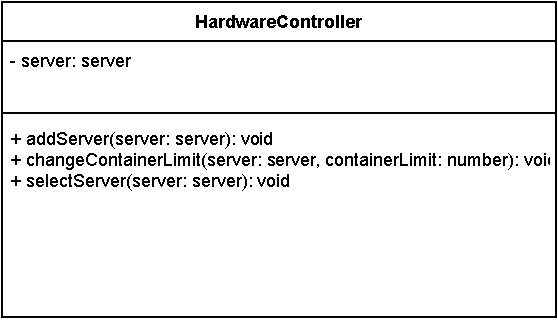
\includegraphics[scale=1]{res/Klassen/HardwareControllerClass.pdf}}
\caption{HardwareController class from class diagram}
\end{figure}

This class is used to surveillance and edit the Hardware of the Server

\begin{methodenv}{Methods}

\method{addServer(server: server): void}

Method adds a Server to the HardwareAdministration

\smallPara{Parameters}
\begin{itemize}
	\item{server:}
	The server that is getting added
\end{itemize}


\method{changeContainerLimit(server: server, containerLimit: number): void}

Method changes the containerlimit of the chosen server to the preferred number.

\smallPara{Parameters}
\begin{itemize}
	\item{server:}
	The server that is getting edited
	\item{containerLimit:}
	the number to which the containerlimit is getting updated to
\end{itemize}


\method{selectServer(server: server): void}

Method selects the server that is getting edited

\smallPara{Parameters}
\begin{itemize}
	\item{server:}
	The server that is getting selected
\end{itemize}
\end{methodenv}




\class{ Server}

\begin{figure}[H]
\centerline{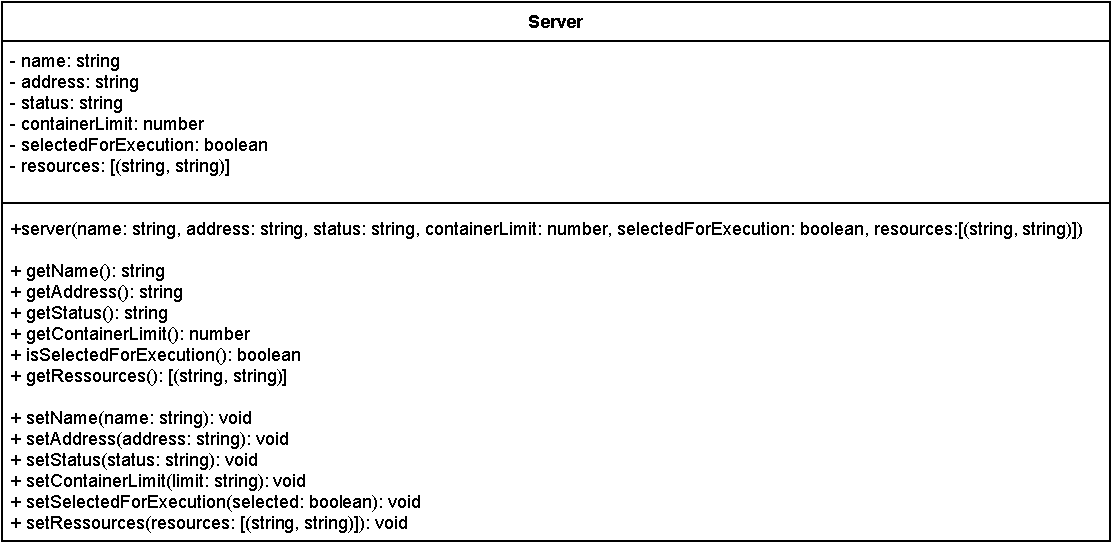
\includegraphics[width=\textwidth]{res/Klassen/ServerClass.pdf}}
\caption{Server class from class diagram}
\end{figure}

This class is used to create a Server object

\begin{methodenv}{Constructor}

\method{server(name: string, address: string, status: string, containerLimit: number, selectedForExecution: boolean, resources: [(string, string)])}

\smallPara{Parameters}

\begin{itemize}
	\item{name:}
	The name of the server
	\item{address:}
	The serveraddress
	\item{status:}
	The server status
	\item{containerLimit:}
	The maximum of containers on the server
	\item{selectedForExecution:}
	Defines if the server is getting used or not
	\item{resources:}
	The servers resources
\end{itemize}
\end{methodenv}

\newpage